%!TEX program = xelatex

\documentclass[11pt,titlepage]{report}
%!TEX root = main.tex

\usepackage[T1]{fontenc}
\usepackage{lmodern}
\usepackage[svgnames]{xcolor}
\usepackage{fontspec} % XeLaTeX required!
\usepackage{graphicx}
\usepackage{circuitikz}
\usepackage{tikz}
\usepackage{pifont}
\usepackage[some]{background}
\usepackage{xltxtra} 
\usepackage{setspace}
\usepackage[absolute]{textpos}
\usepackage[latin1]{inputenc}
\usepackage[english]{babel}
\usepackage{graphicx}
\usepackage{wrapfig}
\usepackage{fullpage}
\usepackage[margin=1in]{geometry}
\usepackage{float}
\usepackage{url}
\usepackage{multicol}
\usepackage{hyperref}
\usepackage{titlepic}
\usepackage{standalone}
\usepackage{siunitx}
\usepackage{booktabs}
\usepackage{amsmath}
\usepackage{unicode-math}
\usepackage{verbatim}
\usepackage{enumitem}
\usepackage{listings}
\usepackage{multirow}
\usepackage{pgfplots}
\pgfplotsset{compat=1.8}
\usepackage{caption} 
\usepackage[parfill]{parskip}
\usepackage{import}
\usepackage[backend=bibtexu,texencoding=utf8,bibencoding=utf8,style=ieee,sortlocale=en_GB,language=auto]{biblatex}
\usepackage[strict,autostyle]{csquotes}
\usepackage[final]{pdfpages}
\usepackage{subcaption}
\usepackage{ifplatform}
%\captionsetup[table]{skip=10pt}


% Fix for includepdf bug in Mac OS X
\newcommand{\insertpdfpath}[1]{
	\ifwindows
	\newcommand{\insertpdf}[2]{\includepdf[pages=##1]{##2}}
	\else
	\newcommand{\insertpdf}[2]{\includepdf[pages=##1]{#1/##2}}
	\fi
}

%set fonts
\setmainfont[Ligatures=TeX]{Myriad Pro}
\setmathfont{Asana Math}
\setmonofont{Lucida Console}

\usepackage{titlesec, color}
\renewcommand{\familydefault}{\sfdefault} %set font family
\renewcommand{\arraystretch}{1.2} %set table vertical spacing
\setlength\parindent{0pt} %no paragraph indent
\hypersetup{ %setup hyperlinks
    colorlinks,
    citecolor=black,
    filecolor=black,
    linkcolor=black,
    urlcolor=black
}

%redesign chapter headings
\definecolor{gray75}{gray}{0.75}
\newcommand{\chapternumber}{\thechapter}
\newcommand{\hsp}{\hspace{20pt}}
\titleformat{\chapter}[hang]{\Huge\bfseries}{\chapternumber\hsp\textcolor{gray75}{|}\hsp}{0pt}{\Huge\bfseries}

%Redefine appendix headers
\renewcommand{\appendixname}{Appendix}
\renewcommand{\appendixtocname}{Appendices}
\renewcommand{\appendixpagename}{Appendices}

%For code listings
\definecolor{black}{rgb}{0,0,0}
\definecolor{browntags}{rgb}{0.65,0.1,0.1}
\definecolor{bluestrings}{rgb}{0,0,1}
\definecolor{graycomments}{rgb}{0.4,0.4,0.4}
\definecolor{redkeywords}{rgb}{1,0,0}
\definecolor{bluekeywords}{rgb}{0.13,0.13,0.8}
\definecolor{greencomments}{rgb}{0,0.5,0}
\definecolor{redstrings}{rgb}{0.9,0,0}
\definecolor{purpleidentifiers}{rgb}{0.01,0,0.01}


\lstdefinestyle{csharp}{
language=[Sharp]C,
showspaces=false,
showtabs=false,
breaklines=true,
showstringspaces=false,
breakatwhitespace=true,
escapeinside={(*@}{@*)},
columns=fullflexible,
commentstyle=\color{greencomments},
keywordstyle=\color{bluekeywords}\bfseries,
stringstyle=\color{redstrings},
identifierstyle=\color{purpleidentifiers},
basicstyle=\ttfamily\small}

\lstdefinestyle{c}{
language=C,
showspaces=false,
showtabs=false,
breaklines=true,
showstringspaces=false,
breakatwhitespace=true,
escapeinside={(*@}{@*)},
columns=fullflexible,
commentstyle=\color{greencomments},
keywordstyle=\color{bluekeywords}\bfseries,
stringstyle=\color{redstrings},
identifierstyle=\color{purpleidentifiers},
}

\lstdefinestyle{matlab}{
language=Matlab,
showspaces=false,
showtabs=false,
breaklines=true,
showstringspaces=false,
breakatwhitespace=true,
escapeinside={(*@}{@*)},
columns=fullflexible,
commentstyle=\color{greencomments},
keywordstyle=\color{bluekeywords}\bfseries,
stringstyle=\color{redstrings},
identifierstyle=\color{purpleidentifiers}
}

\lstdefinestyle{vhdl}{
language=VHDL,
showspaces=false,
showtabs=false,
breaklines=true,
showstringspaces=false,
breakatwhitespace=true,
escapeinside={(*@}{@*)},
columns=fullflexible,
commentstyle=\color{greencomments},
keywordstyle=\color{bluekeywords}\bfseries,
stringstyle=\color{redstrings},
identifierstyle=\color{purpleidentifiers}
}

\lstdefinestyle{xaml}{
language=XML,
showspaces=false,
showtabs=false,
breaklines=true,
showstringspaces=false,
breakatwhitespace=true,
escapeinside={(*@}{@*)},
columns=fullflexible,
commentstyle=\color{greencomments},
keywordstyle=\color{redkeywords},
stringstyle=\color{bluestrings},
tagstyle=\color{browntags},
morestring=[b]",
  morecomment=[s]{<?}{?>},
  morekeywords={xmlns,version,typex:AsyncRecords,x:Arguments,x:Boolean,x:Byte,x:Char,x:Class,x:ClassAttributes,x:ClassModifier,x:Code,x:ConnectionId,x:Decimal,x:Double,x:FactoryMethod,x:FieldModifier,x:Int16,x:Int32,x:Int64,x:Key,x:Members,x:Name,x:Object,x:Property,x:Shared,x:Single,x:String,x:Subclass,x:SynchronousMode,x:TimeSpan,x:TypeArguments,x:Uid,x:Uri,x:XData,Grid.Column,Grid.ColumnSpan,Click,ClipToBounds,Content,DropDownOpened,FontSize,Foreground,Header,Height,HorizontalAlignment,HorizontalContentAlignment,IsCancel,IsDefault,IsEnabled,IsSelected,Margin,MinHeight,MinWidth,Padding,SnapsToDevicePixels,Target,TextWrapping,Title,VerticalAlignment,VerticalContentAlignment,Width,WindowStartupLocation,Binding,Mode,OneWay,xmlns:x}
}

\lstdefinestyle{matlab}{
language=Matlab,
showspaces=false,
showtabs=false,
breaklines=true,
showstringspaces=false,
breakatwhitespace=true,
escapeinside={(*@}{@*)},
columns=fullflexible,
commentstyle=\color{greencomments},
keywordstyle=\color{bluekeywords}\bfseries,
stringstyle=\color{purpleidentifiers},
identifierstyle=\color{purpleidentifiers}
}

%defaults
\lstset{
basicstyle=\ttfamily\small,
extendedchars=false,
numbers=left,
numberstyle=\ttfamily\tiny,
stepnumber=1,
tabsize=4,
numbersep=5pt
}
\addbibresource{../../library/bibliography.bib}

\begin{document}

\chapter{Control}
\label{ch:control}
\section{Introduction}
This chapter will describe the methodology we used to control KITT's position, to drive KITT to a certain location on the playing field, also known as a waypoint. To achieve this seemingly easy task, we invented a method which we call \textit{reduction of dimensionality}. Controlling KITT to a given position can be seen as a two-dimensional problem. Consider KITT a black box, then the inputs are given by the driving and steering excitation, and the output by the current position. One could create a model of the whole system. However, this model would be non-linear and therefore hard to control. A better approach seemed to divide the complex two-dimensional problem into two less complicated one-dimensional problems; \textbf{(1)}, controlling KITT's speed in a way that KITT stops at the specified target and \textbf{(2)}, controlling KITT's angle in a way that KITT drives a specified trajectory. This concept is shown in Figure~\ref{fig:ctrl-reduction}. \textbf{(1)} and \textbf{(2)} are carried out by respectively the distance and angle controller. 

\begin{figure}[H]
	\centering
	\begin{tikzpicture}[node distance=5cm, auto]
		% Nodes
		\node [rectangle] (kitt) {KITT} (0,0);

		% Input edges
		\path [line, ->, yshift=0.5cm] (-8,0) -- node [anchor=center,fill=white] {Drive excitation signal} ([yshift=0.5cm]kitt.west);
		\path [line, ->, yshift=-0.5cm] (-8,0) -- node [anchor=center,fill=white] {Steering excitation signal} ([yshift=-0.5cm]kitt.west);

		% Output edges
		\path [line, ->] (kitt.east) -- node [anchor=center,fill=white] {Position} (8,0);

		% Bottom thing 1
		\begin{scope}[yshift=-5cm]
			% Nodes
			\node [rectangle, minimum height=3em] (kitt2) {KITT} (0,0);

			% Input edges
			\path [line, ->] (-8,0) -- node [anchor=center,fill=white] {Drive excitation signal} (kitt2.west);

			% Output edges
			\path [line, ->] (kitt2.east) -- node [anchor=center,fill=white] {Distance to target} (8,0);
		\end{scope}

		% Bottom thing 1
		\begin{scope}[yshift=-6.5cm]
			% Nodes
			\node [rectangle, minimum height=3em] (kitt3) {KITT} (0,0);

			% Input edges
			\path [line, ->] (-8,0) -- node [anchor=center,fill=white] {Steering excitation signal} (kitt3.west);

			% Output edges
			\path [line, ->] (kitt3.east) -- node [anchor=center,fill=white] {Angle} (8,0);
		\end{scope}
		
		% Connection
		\path [line, ->, line width=5pt,] ([yshift=-0.5cm]kitt.south) -- node [anchor=center,fill=white] {\Large Reduction of dimensionality} ([yshift=0.5cm]kitt2.north);
	\end{tikzpicture}
	\caption{Reduction of dimensionality}
	\label{fig:ctrl-reduction}
\end{figure}


 The whole methodology can be divided in two processes; \textit{routing} and \textit{controlling}. Routing takes care of planning the trajectory KITT is going to drive, and controlling manages KITT to drive, following the trajectory, to the waypoint. Figure~\ref{fig:ctrl-overview} shows a complete overview. This overview makes clear that the whole controller determines KITT's actuator excitation data given a current location, angle, which is the direction in which KITT drives, waypoint and sensor data.

\begin{figure}[H]
	\begin{center}
		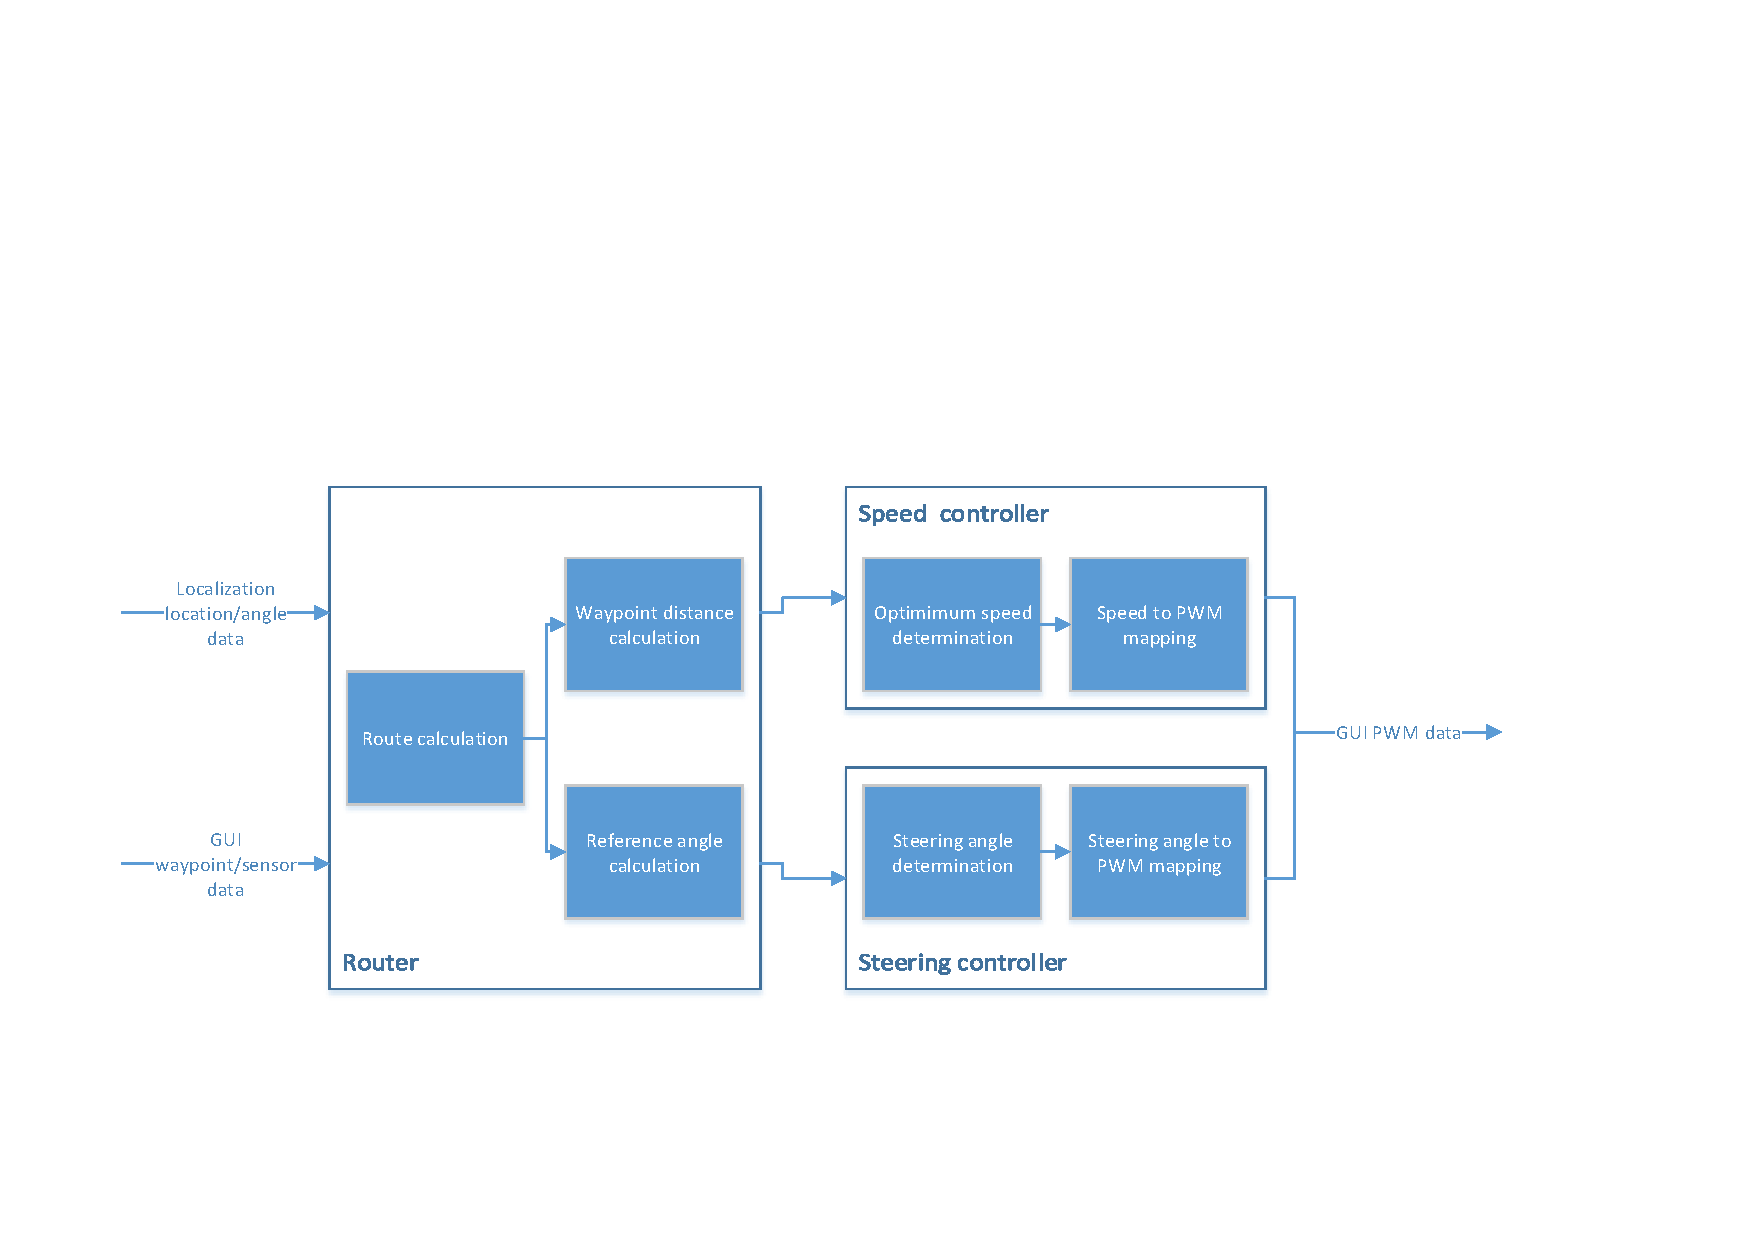
\includegraphics[width=\linewidth]{resource/control-overview.pdf}
	\end{center}
	\caption{Overview of the control}
	\label{fig:ctrl-overview}
\end{figure}

First, we will describe the way routing is done. Second, controlling will be given some thought. This chapter will be concluded with some final thoughts.

\section{Routing}
\subsection{Introduction}
The \textit{router}, the submodule of control that takes care of the routing process, plans the trajectory KITT is going to drive. Essentially, the router determines in what direction KITT should drive, expressed as a reference angle, and the distance KITT still has to drive to the current waypoint, given the current waypoint, angle, location and sensor data. KITT should also not collide with obstacles. Therefore, the router must consider the sensor data when determining the reference angle and distance. A schematic representation is given in Figure~\ref{fig:ctrl-router}.

\begin{figure}[H]
	\centering
	\begin{tikzpicture}[node distance=5cm, auto]
		% Nodes
		\node [rectangle] (router) {Router} (0,0);

		% Input edges
		\path [line, ->, yshift=0.75cm] (-8,0) -- node [anchor=center,fill=white] {Sensor data} ([yshift=0.75cm]router.west);
		\path [line, ->] (-8, 0) -- node [anchor=center,fill=white] {Current waypoint} (router.west);
		\path [line, ->, yshift=-0.75cm] (-8,0) -- node [anchor=center,fill=white] {Current angle and location} ([yshift=-0.75cm]router.west);

		% Output edges
		\path [line, ->, yshift=0.5cm] ([yshift=0.5cm]router.east) -- node [anchor=center,fill=white] {Current distance} (8,0);
		\path [line, ->, yshift=-0.5cm] ([yshift=-0.5cm]router.east) -- node [anchor=center,fill=white] {Reference angle} (8,0);
	\end{tikzpicture}
	\caption{Router}
	\label{fig:ctrl-router}
\end{figure}

The router operates in two different modes; \textit{trajectory planning} and \textit{obstacle avoidance}. When the sensor data indicates that the path is clear, the router plans the trajectory to reach the current waypoint as fast as possible. However, when an obstacle is detected, the router fully focuses on avoiding that obstacle. This section will describe trajectory planning and obstacle avoidance separately.

\subsubsection{Trajectory planning}
Let KITT's current location be denoted by $\vec{x}$, the current waypoint by $\vec{w}$ and KITT's current angle by $\theta$. The goal is to determine the angle $\theta_{\text{ref}}$ which KITT should reach, to drive as fast as possible to the current waypoint, and the distance left to this waypoint $d$. The ideal direction in which KITT should drive, expressed as an unit direction vector $\vec{v}$, is given by
\[
	\vec{v} = \frac{\vec{w} - \vec{x}}{||\vec{w} - \vec{x}||}.
\]
The absolute angle difference between KITT's ideal angle and KITT's current angle $\theta_{\text{diff}}$ is then given by
\[
	\theta_{\text{diff}} = ||\theta_{\text{ref}} - \theta|| = \operatorname{arccos}\left( \tr{\begin{bmatrix}
		\cos{(\theta)} & \sin{(\theta)}
	\end{bmatrix}} \cdot \vec{v} \right).
\]
To determine whether $\theta_{\text{ref}}$ has to be substracted or added to $\theta$ to determine the ideal reference angle, the sign of inner product of a vector orthogonal to the ideal direction vector of KITT and the actual direction vector of KITT is evaluated. Therefore, $\theta_{\text{ref}}$ is given by
\[
	\theta_{\text{ref}} = \theta + \operatorname{sign}\left(\left( \begin{bmatrix}
		0 & 1 \\
		-1 & 0
	\end{bmatrix} \vec{v} \right) \cdot \begin{bmatrix}
		\cos{(\theta)} \\
		\sin{(\theta)}
	\end{bmatrix}\right) \theta_{\text{diff}}.
\]
The reason we try to express $\theta_{\text{ref}}$ as function of $\theta$ and $\theta_{\text{diff}}$ and not simply of $\vec{v}$, is that this expression easily translates to a steering angle. Finally, we limit $\theta_{\text{ref}}$ to account for the maximum angle at which KITT can turn. The way the controlling process works, is that KITT first turns, which means following its turning circle, until its direction vector is tangent with $\vec{v}$ -- this location is called the tangent point $\vec{p}$ -- and then drives in a straight line to the current waypoint. This situation is depicted in Figure~\ref{fig:ctrl-route-trajectory}.

\begin{figure}[H]
	\centering
	\begin{tikzpicture}[node distance = 6.5cm, auto]
		\draw [black] (0,-1) -- node [anchor=south, pos=0.3, rotate=90] {$y \rightarrow$} (0,5);
		\draw [black] (-1,0) -- node [anchor=north, pos=0.2] {$x \rightarrow$} (8,0);

		\begin{scope}[yshift=-1cm]
			\draw [red, fill=red] (3,3) circle [radius=0.1] node [black,xshift=0.3cm] {$\vec{x}$};
			
			\draw [red, line width=1pt] (2,3) circle [radius=1];
			\draw [black, fill=black] (2,3) circle [radius=0.05] node [black,xshift=-0.3cm] {$\vec{t}_1$};
			\draw [line, <->, black] (2,3) -- node [black] {$R$} (3,3);
			\draw [red, line width=1pt] (4,3) circle [radius=1];
			\draw [black, fill=black] (4,3) circle [radius=0.05] node [black,xshift=0.3cm] {$\vec{t}_2$};
			\draw [line, ->, >=triangle 45, black, thick, line width=1pt] (3,3) -- (3,4);
			\draw [line, ->, line width=1pt, red] (4,4) -- (7,4);
			\draw [black, fill=black] (7,4) circle [radius=0.05] node [black,xshift=0.3cm] {$\vec{w}$};
			\draw [black, fill=black] (4,4) circle [radius=0.05] node [black,yshift=0.3cm] {$\vec{p}$};
			\draw [black, <->, >=latex] (3.7,3) arc [radius=0.3, start angle=180, end angle=90] node [xshift=-0.4cm,yshift=0.2cm] {$\Delta \alpha$};
		\end{scope}
	\end{tikzpicture}
	\caption{Depiction of KITT's trajectory}
	\label{fig:ctrl-route-trajectory}
\end{figure}

The turning point $\vec{t}$ around which KITT turns until it is tangent with $\vec{v}$ is given by
\[
	\vec{t}_{1,2} = \vec{x} \pm R \begin{bmatrix}
		0 & -1 \\
		1 & 0
	\end{bmatrix} \begin{bmatrix}
		\cos{(\theta)} \\ \sin{(\theta)}
	\end{bmatrix},
\]
\[
	\vec{t} = \underset{\vec{t}_i, i \in \{1,2\}}{\operatorname{min}} ||\vec{t}_i - \vec{w} ||,
\]
where $R$ denotes the turning radius. The distance $d$ now consists of two parts; the distance $d_1$ KITT turns from $\vec{x}$ to $\vec{p}$, and the distance $d_2$ from $\vec{p}$ to $\vec{w}$. $d_2$ is simply given by
\[
	d_2 = ||\vec{p}-\vec{w}|| = \sqrt{R^2 + ||\vec{t} - \vec{w}||^2}.
\]
To determine $d_1$, we have to know the position $\vec{p}$. Logically thinking, two possible, approximate -- let us not overcomplicate the problem -- locations of $\vec{p}$ are given by
\[
	\vec{p}_{1,2} = \vec{t} \pm R \begin{bmatrix}
		0 & -1 \\
		1 & 0
	\end{bmatrix} \vec{v}.
\]
Determining whether $\vec{p} = \vec{p}_1$ or $\vec{p} = \vec{p}_2$ requires to know if KITT turns towards $\vec{p}_1$ or $\vec{p}_2$. First, the direction in which KITT drives, relative to the orientation of its turning circle, can be checked by evaluating the sign of
\[
	\left( \begin{bmatrix}
		0 & -1 \\
		1 & 0
	\end{bmatrix} \left( \vec{t} - \vec{x} \right) \right) \cdot \begin{bmatrix}
		\cos{(\theta)} \\
		\sin{(\theta)}
	\end{bmatrix}.
\]
Then, doing a coordinate transformation by letting $\vec{t}$ be $(0,0)$ and comparing the angles of $\vec{p}_1$ and $\vec{p}_2$ relative to the positive x-axis allow us to determine $\vec{p}$. With these angles, the angle $\Delta \alpha$ of its turning circle which KITT has to drive to reach $\vec{p}$ can be calculated. $d_1$ is then given by
\[
	d_1 = \Delta \alpha R.
\]
This concludes calculating the reference angle $\theta_{\text{ref}}$ KITT should reach, to drive as fast as possible to the current waypoint the distance $d$ left to this waypoint.

\subsection{Obstacle avoidance}
When KITT comes across an obstacle, the sensors detect the frontal distances to this object. Obstacle avoidance is based on the follow rule; go the easiest way around the object while keeping a certain clearance $c$. Let the left sensor distance be given by $s_l$ and the right sensor distance by $s_r$. Figure~\ref{fig:ctrl-route-obstacle} depicts a situation in which KITT comes across an obstacle.

\begin{figure}[H]
	\centering
	\begin{tikzpicture}[node distance = 6.5cm, auto]
		\draw [black] (0,-1) -- node [anchor=south, pos=0.2, rotate=90] {$y \rightarrow$} (0,8);
		\draw [black] (-1,0) -- node [anchor=north, pos=0.2] {$x \rightarrow$} (8,0);

		\draw [black] (2,1) rectangle node [anchor=center] {KITT} (3,2);
		\draw [line width=5pt] (1,4) -- (4,7);
		\draw [line, <->, black] (2.2,2) -- node [anchor=center,fill=white] {$s_l$} (2.2,5.2);
		\draw [line, <->, black] (2.8,2) -- node [anchor=center,fill=white,pos=0.42] {$s_r$} (2.8,5.8);
		\draw [line, red] (2.5,2) -- (2.5,5.5);
		\draw [line, <->, red] (2.8,5.8) -- node [anchor=center,fill=white] {$c$} (5.8,5.8); 
		\draw [line, red] (2.8,2) -- (5.8,5.8);
		\draw [red, <->, >=latex] (2.5,4.62) arc [radius=3, start angle=90, end angle=51.7] node [red, yshift=0.8cm, xshift=-.8cm] {$\phi$};
	\end{tikzpicture}
	\caption{Depiction of KITT avoiding an obstacle}
	\label{fig:ctrl-route-obstacle}
\end{figure}

Let the distance between both sensors on KITT be given by $L$, then $\phi$ is given by
\[
	\phi = \operatorname{arctan}\left(\frac{c}{L/2+\operatorname{max}(s_{r,l})}\right).
\]
Using the information which sensor's value is maximal, and then accordingly adding or substracting $\phi$ to or from $\theta$ yields $\theta_{\text{ref}}$. Finally, we again limit $\theta_{\text{ref}}$ to account for the maximum angle at which KITT can turn. 
% Opbouw:
% - Inleiding: weten afstand, gewenste afstand, hoek, gewenste hoek, hoe PWM waardes bepalen zodat bereikt wordt
% reductie dimensionaliteit, twee onafhankelijk werkende systemen
% - Controllers:
% * Distance controller
% * Angle controller
% - Excitation mapping
% - Solving the models
\section{Controlling}
\subsection{Introduction}
At this point we assume certain things to be known; the current distance to the next waypoint, KITT's current angle and KITT's ideal angle, expressed as a reference angle. A system must be designed which controls KITT in a way that the distance to the next waypoint reduces to zero. In other words, KITT needs to be controlled to the next waypoint.

This section will discuss the implementation of our so-called reduction of dimensionality. First, the design of the distance and angle controller will be discussed. Second, the mapping of the controllers' output to a by KITT understandable signal will be explained. At last, the actual implementation will be talked through.


\subsection{Distance controller}
\subsubsection{Introduction}
The distance controller takes care of KITT autonomously driving to and then stopping at a specified distance. Note that the distance controller does \textit{not} control the direction in which KITT is driving. The whole controller is based on the following assumption; speeding up KITT to a constant speed will cause the distance to its target to decrease linearly. The controller consists of two components; the \textit{observer} and the \textit{compensator}. We will explain both of these in further detail.

\subsubsection{Observer design}
The distance controller must have knowledge of the current distance and speed of the car to be able to successfully control KITT. Generalizing, we can say that the controller must have knowledge of the current \textit{state} of KITT. The observer's task is to keep track of the internal state. This internal state consists of a linear combination of all generalized positions and momenta of respectively all inductive and capacitive components of the system. If we consider KITT a state-space model, we can define its inputs and an output. Figure~\ref{fig:ctrl-model} represents this line of thought schematically.

\begin{figure}[H]
	\centering
	\begin{tikzpicture}[node distance = 7cm, auto]
		% Nodes
		\node [] (input) {};
		\node [rectangle, right of=input] (kitt) {KITT \\[1em] $\begin{bmatrix} \dot{\vec{x}} \\ \vec{y} \end{bmatrix} = \begin{bmatrix} \mat{A} & \mat{B} \\ \mat{C} & \mat{D} \end{bmatrix} \begin{bmatrix} \vec{x} \\ \vec{u} \end{bmatrix}$};
		\node [right of=kitt] (output) {};
		% Edges
		\path [line, ->] (input) -- node [anchor=center,fill=white] {$\vec{u}$ (drive excitation signal)} (kitt);
		\path [line, ->] (kitt) -- node [anchor=center,fill=white] {$\vec{y}$ (distance)} (output);
	\end{tikzpicture}
	\caption{State-space based model of KITT}
	\label{fig:ctrl-model}
\end{figure}

The observer observes the input $\vec{u}$ and output $\vec{y}$ and determines, by doing that, the internal state $\vec{x}$ of KITT. We modelled the observer by making also use of a state-space representation. Figure~\ref{fig:ctrl-model-observer} shows the state-space model of the observer and its interconnection to KITT's state-space model. Logically thinking, the observer must obey two constraints; \textbf{(1)}, the internal state $\hat{\vec{x}}$ of the observer must converge to $\vec{x}$ if $t \to \infty$ and \textbf{(2)}, if $\hat{\vec{x}} = \vec{x}$, then the states should not diverge. To fulfil \textbf{(1)}, we introduce a feedback matrix $\mat{L}$, and to satisfy \textbf{(2)}, the system, input-, output- and feed-through matrix of the observer should match KITT's. We can show constraint \textbf{(1)} by evaluating the error $\vec{e}=\vec{x}-\hat{\vec{x}}$. Inspecting $\dot{\vec{e}}$ yields 
\begin{equation} \label{eq:ctrl-err}
	\dot{\vec{e}}=\dot{\vec{x}} - \dot{\hat{\vec{x}}} = \mat{A} (\vec{x} - \hat{\vec{x}}) - \mat{L} (\vec{y} - \hat{\vec{y}}) = (\mat{A} - \mat{L} \mat{C}) (\vec{x} - \hat{\vec{x}}) = (\mat{A} - \mat{L}\mat{C}) \vec{e}.
\end{equation}
Equation~\ref{eq:ctrl-err} tells us the the system is observable, if $\mat{A} - \mat{L}\mat{C}$ renders $\vec{e}$ asymptotically stable. This defines the observability of the pair $(\mat{C}, \mat{A})$. The duality between observability and controllability tells us that $(\mat{C},\mat{A})$ is observable if $(\tr{\mat{A}},\tr{\mat{C}})$ is controllable.

\begin{figure}[H]
	\centering
	\begin{tikzpicture}[node distance = 6.5cm, auto]
		% Nodes
		\node [rectangle] (kitt) at (6,0) {KITT \\[1em] $\begin{bmatrix} \dot{\vec{x}} \\ \vec{y} \end{bmatrix} = \begin{bmatrix} \mat{A} & \mat{B} \\ \mat{C} & \mat{D} \end{bmatrix} \begin{bmatrix} \vec{x} \\ \vec{u} \end{bmatrix}$};
		\node [rectangle, text width=11em] (observer) at (10,4) {Observer \\[1em] $\begin{bmatrix} \dot{\hat{\vec{x}}} \\ \hat{\vec{y}} \end{bmatrix} = \begin{bmatrix} \mat{A} & \mat{B} & \mat{L} \\ \mat{C} & \mat{D} & 0 \end{bmatrix} \begin{bmatrix} \hat{\vec{x}} \\ \vec{u} \\ \vec{y} - \hat{\vec{y}} \end{bmatrix}$};

		% Coordinates
		\coordinate (input) at (0,4);
		\coordinate (input_split) at (1,4);
		\coordinate (output) at (16,4);

		% Edges
		\path [line, ->] (input) -- node [anchor=center,fill=white] {$\vec{u}$ (drive excitation signal)} (observer.west);
		% \path (input) edge [->, pos=0.3] node {$\vec{u}$ (drive excitation signal)} (observer.west);
		\path [line, ->] (kitt.east) -| node [anchor=center,fill=white,pos=0.7] {$\vec{y}$ (position)} (observer.south);
		\path [line, ->] (input_split) |- node [] {} (kitt.west);
		\path [line, ->] (observer.east) -- node [anchor=center,fill=white] {$\hat{\vec{x}}$ (internal state)} (output);
	\end{tikzpicture}
	\caption{State-space based model of KITT and the observer}
	\label{fig:ctrl-model-observer}
\end{figure}

\begin{figure}[H]
	\centering
	\begin{tikzpicture}[node distance=2cm]
		\bgComponentNoBond{bat}{$S_e:v$}
		\bgComponent{}{1-1}{1}{right of=}{bat}{inbond}
		\bgComponent{}{ind}{$I:L$}{above of=}{1-1}{inbond}
		\bgComponent{}{res1}{$R:R$}{below of=}{1-1}{inbond}

		\bgComponentWithBondLabel{}{gy}{GY}{right of=}{1-1}{inbond}{}{$e_1=e$}{$f_1=i$}

		\bgComponentWithBondLabel{node distance=3cm}{loss}{TF}{right of=}{gy}{inbond}{}{$k_t f_1=\tau_m$}{$k_t^{-1} e_1=\omega_m$}
		\bgComponentWithBondLabel{node distance=3cm}{conv}{TF}{right of=}{loss}{inbond}{}{$k_g \tau_m=\tau_w$}{$k_g^{-1} \omega_m = \omega_w$}
		\bgComponentWithBondLabel{node distance=3cm}{1-2}{1}{right of=}{conv}{inbond}{}{$r_w^{-1} \tau_w=F$}{$r_w \omega_w=v$}


		\bgComponent{}{mass}{$I:m$}{above of=}{1-2}{inbond}
		\bgComponent{}{res2}{$R:\rho$}{right of=}{1-2}{inbond}
	\end{tikzpicture}
	\caption{Bond graph representation of KITT's model}
	\label{fig:ctrl-bond}
\end{figure}

The only thing which remains is determining the system matrices $\mat{A}$, $\mat{B}$, $\mat{C}$ and $\mat{D}$ and  the feedback matrix $\mat{L}$. For the system matrices, we use the bond graph depicted in Figure~\ref{fig:ctrl-bond} to derive the state-space model shown in Equation~\ref{eq:ctrl-bond-model}. Here the battery voltage is denoted by $v$, the inductance of the motor by $L$, the internal resistance of the motor by $R$, the motor constant by $k_t$, the gear constant by $k_g$, the radius of the wheels by $r_w$, the mass of KITT by $m$, the rolling resistance coefficient by $\rho$ and $k_t k_g/r_w$ by $r$. A generalized notation of the position and the velocity is used. The observability matrix $\mathcal{O}$ and the controllability matrix $\mathcal{C}$ reveal that the system is both observable and controllable.

\begin{align} \label{eq:ctrl-bond-model}
	\dot{\vec{x}} = \frac{d}{dt}
	\begin{bmatrix}
		q_m \\
		f_m \\
		f_L
	\end{bmatrix} &= \mat{A} \vec{x} + \mat{B} \vec{u} =
	\begin{bmatrix}
		0 & 1 & 0 \\
		0 & -\frac{\rho}{m} & \frac{r}{m} \\
		0 & -\frac{r}{L} & -\frac{R}{L}
	\end{bmatrix}
	\begin{bmatrix}
		q_m \\
		f_m \\
		f_L
	\end{bmatrix} +
	\begin{bmatrix}
		0 \\
		0 \\
		\frac{1}{L}
	\end{bmatrix} v \\
	\vec{y} = q_m &= \mat{C} \vec{x} + \mat{D} \vec{u} =
	\begin{bmatrix}
		1 & 0 & 0
	\end{bmatrix}
	\begin{bmatrix}
		q_m \\
		f_m \\
		f_L
	\end{bmatrix}
\end{align}

To determine the poles introduced by the feedback matrix $\mat{L}$, denoted by $\lambda_1$ and $\lambda_2$, we define a measure of performance for each pair of poles $(\lambda_1,\lambda_2)$. We let the observer track measurement data which consisted of the drive excitation $\vec{u}$ and distances measured $\vec{y}$. The observer then produces the tracked distance $\mat{C} \hat{\vec{x}} = \hat{\vec{y}}$. Let the time interval between $\vec{y}_n$ and $\vec{y}_{n+1}$ is $\Delta T$. We define the error $e_i$ of experiment $i$ to be

\begin{equation*} \label{ctrl:err}
	e_i = \int_{0}^{t_f} || \vec{y}(t) - \hat{\vec{y}}(t) || dt = \sum_{0}^{N} ||\vec{y}_n - \hat{\vec{y}}_n || \Delta T.
\end{equation*}

\begin{figure}[H]
	\begin{center}
		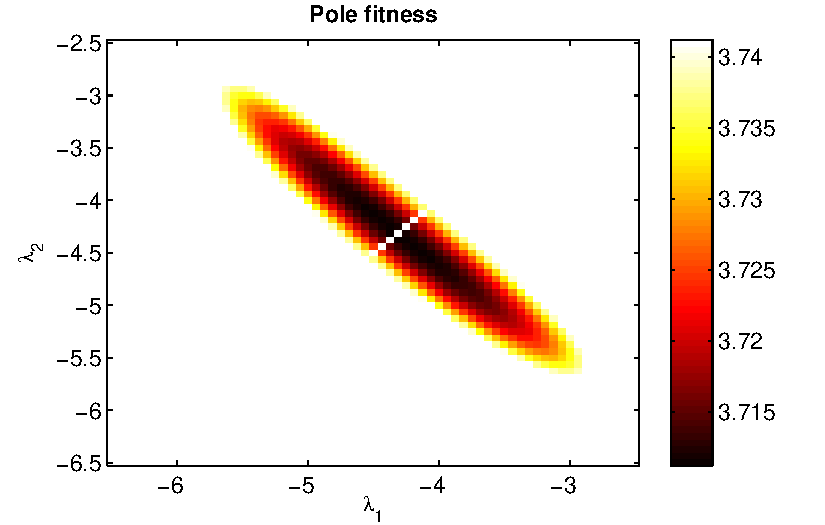
\includegraphics[width=.7\linewidth]{resource/pole-fitness.pdf}
	\end{center}
	\caption{Performance of different pairs of poles of the observer, lower is better}
	\label{fig:ctrl-poles}
\end{figure}

Figure~\ref{fig:ctrl-poles} shows the error of many different pairs of poles. It is clear that there exists a maximum at $\lambda_1=\lambda_2$. This is obvious, because using Jordan's normal form, one can show that when $\lambda_1 = \lambda_2>0$, 
$\vec{e}$ is critically damped. Also, $\lambda_1 = \lambda_2$ renders the system matrix non-diagonalizable, which explains the presence of the white line at every point where $\lambda_1=\lambda_2$. At last, the reason the maximum is not located at $(-\infty,-\infty)$, which corresponds with the highest convergence of the observer possible, is because we are also dealing with latency, meaning that oscillations of $\vec{e}$ can be caused by poles too large.  

\subsubsection{Compensator design}
Lets go back to Figure~\ref{fig:ctrl-model} and say we actually know the internal state $\vec{x}$. To derive a method to control our state-space model of KITT, we define a reference state $\vec{x}_{\text{ref}} = \tr{\begin{bmatrix*}
	d_{\text{ref}} & 0 & 0 
\end{bmatrix*}}$. Let us now introduce the feedback law $\vec{u} = -\mat{K}(\vec{x}-\vec{x}_{\text{ref}})$. Rewriting the state-space model equations yields

\begin{equation} \label{eq:ctrl-comp}
	\dot{\vec{x}} = (\mat{A} - \mat{B} \mat{K}) \vec{x} + \mat{B} \mat{K} \vec{x}_{\text{ref}}.
\end{equation}

If we argue that $\mat{A} - \mat{B} \mat{K}$ renders the system asymptotically stable, then rewriting Equation~\ref{eq:ctrl-comp} using $\dot{\vec{x}} \to 0$ when $t \to \infty$ yields

\begin{align*}
	(\mat{B} \mat{K} - \mat{A}) \vec{x} &= \mat{B} \mat{K} \vec{x}_{\text{ref}}.
\end{align*}

Further simplifying using Equation~\ref{eq:ctrl-bond-model} yields $q_m = d_{\text{ref}}$ and $f_m = f_L = 0$. This means that the model shown in Figure~\ref{fig:ctrl-model} converges to a state where KITT is not moving at a specified distance $d_{\text{ref}}$. In other words, we specify the position at which KITT stops moving, which is exactly what we want. The only thing which remains, is determining the poles of $\mat{A} - \mat{B} \mat{K}$. We want KITT to stop at our specified position as fast as possible, without overshooting. Therefore, KITT must critically damped converge to a distance $d_{\text{ref}}$. If $\lambda_1$ and $\lambda_2$ are the eigenvalues of $\mat{A} - \mat{B} \mat{K}$, then $\lambda_1$ and $\lambda_2$ where $\lambda_1 = \lambda_2 = \lambda < 0$ must as negative as possible. The exact value of $\lambda$ depends on the latency we are dealing with. We adjusted these eigenvalues on-the-go to achieve an optimized result.

\subsubsection{Distance controller design}
Putting together the observer and the compensator together yields the whole distance controller, that is able to control KITT to a specified distance $d_{\text{ref}}$. This closed-loop system is depicted in Figure~\ref{fig:ctrl-dist-controller}. Note that we discussed the design of the observer and compensator as if they could be designed separately. This is exactly what the separation principle states. 

\begin{figure}[H]
	\centering
	\begin{tikzpicture}[node distance = 6.5cm, auto]
		% Nodes
		\node [rectangle] (kitt) at (0,0) {KITT \\[1em] $\begin{bmatrix} \dot{\vec{x}} \\ \vec{y} \end{bmatrix} = \begin{bmatrix} \mat{A} & \mat{B} \\ \mat{C} & 0 \end{bmatrix} \begin{bmatrix} \vec{x} \\ \vec{u} \end{bmatrix}$};
		\node [rectangle, text width=14em] (controller) at (0,4) {Controller \\[1em] $\begin{bmatrix} \dot{\hat{\vec{x}}} \\ \hat{\vec{y}} \end{bmatrix} = \begin{bmatrix} \mat{A}-\mat{B}\mat{K} & \mat{B}\mat{K} & \mat{L} \\ \mat{C} & 0 & 0 \end{bmatrix} \begin{bmatrix} \hat{\vec{x}} \\ \vec{x}_{ref} \\ \vec{y} - \hat{\vec{y}} \end{bmatrix}$};

		% Edges
		\path [line, ->] (controller.west) -| node [anchor=center,fill=white,pos=1] {$\vec{u}$ (drive excitation signal)} (-5,2) |- (kitt.west);
		\path [line, ->] (kitt.east) -| node [anchor=center,fill=white,pos=1] {$\vec{y}$ (position)} (5,2) |- (controller.east);
		\path [line, ->] (0,7) -- node [anchor=center,fill=white] {$\vec{x}_{ref}$ (reference state)} (controller.north);
	\end{tikzpicture}
	\caption{State-space based distance controller of KITT}
	\label{fig:ctrl-dist-controller}
\end{figure}

\subsection{Angle controller}
\subsubsection{Introduction}
The distance controller was based on the assumption that a constant speed of KITT causes a linearly decreasing distance. This can only be realized if KITT drives the predicted trajectory. It is the angle controller's responsibility that KITT drives this trajectory by controlling the angle of the wheels. Before we can design an angle controller, we must find a relationship between the angle of the wheels and the rate at which KITT turns.

\subsubsection{Analysis}
Let us consider a car with distance $L$ between both wheel axes. The rear axis of the car is located at $(0,0)$ and the front axis at $(L,0)$ in a way that they are parallel to each other. The front wheels are turned an angle $\phi$ relative to the positive $x$-axis. If the car drives at a speed $v$, then approximately, after a very small time $\Delta t$, the rear axis is located at $(v \cos{(\phi)}\Delta t,0)$ and the front axis at $(L+v \cos{(\phi)}\Delta t,v \sin{(\phi)}\Delta t)$. The situation is sketched in Figure~\ref{fig:ctrl-angle-sketch}.

\begin{figure}[H]
	\centering
	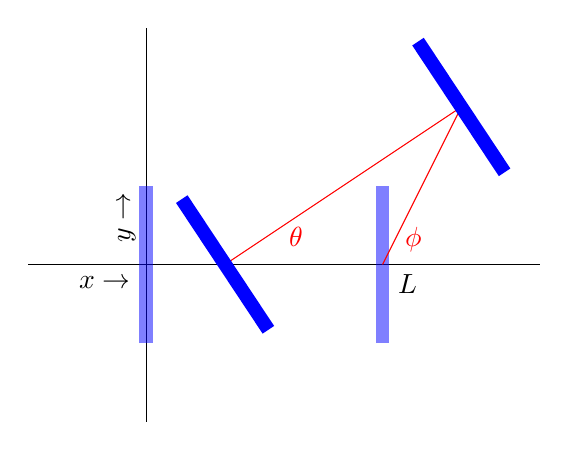
\begin{tikzpicture}[node distance = 6.5cm, auto]
		\draw [black] (0,-2) -- node [anchor=south, pos=0.52, rotate=90] {$y \rightarrow$} (0,3);
		\draw [black] (-1.5,0) -- node [anchor=north, pos=0.15] {$x \rightarrow$} (5,0);

		% Wheel axis
		\draw [blue, line width=5pt, opacity=0.5] (0,-1) -- (0,1);
		\draw [blue, line width=5pt, opacity=0.5] (3,-1) -- node [anchor=west,text=black,yshift=-0.25cm,opacity=1] {$L$} (3,1);

		\draw [red] (3,0) -- node [anchor=north,pos=0.3,xshift=0.1cm] {$\phi$} (4,2);
		\draw [red] (1,0) -- node [anchor=north,pos=0.3] {$\theta$} (4,2);

		\draw [blue, line width=5pt] (0.45,0.83) -- (1.55,-0.83);
		\draw [blue, line width=5pt] (3.45,2.83) -- (4.55,1.17);

	\end{tikzpicture}
	\caption{Approximation of KITT's movement}
	\label{fig:ctrl-angle-sketch}
\end{figure}

The car was first parallel to the positive $x$-axis. Therefore, if $\theta$ denotes the angle of the car relative to the positive $x$-axis,
\[
	\theta(t) = 0
\]
and
\[
	\theta(t+\Delta t)=\arctan{\left(\frac{v \sin{(\phi)}\Delta t}{L}\right)}.
\]
We can now evaluate $\dot{\theta}(t)$ by evaluating the limit
\begin{align}
	\dot{\theta}(t) &= \lim_{\Delta t \rightarrow 0} \frac{\theta(t+\Delta t)-\theta(t)}{\Delta t} \nonumber \\
	&= \lim_{\Delta t \rightarrow 0} \frac{\arctan{\left(\frac{v \sin{(\phi)}\Delta t}{L}\right)}}{\Delta t} \nonumber \\
	&= \lim_{\Delta t \rightarrow 0} \left(1+\frac{v^2 \sin{(\phi)}\Delta t^2}{L^2}\right)^{-1}\frac{v \sin{(\phi)}}{L} \quad \quad \text{(L'H\^opital's rule)} \nonumber \\
	&= \frac{v \sin{(\phi)}}{L}. \label{eq:steering-derivative}
\end{align}
We have now found a relation between rate at which KITT turns and the angle of KITT's wheels. The other thing which remains is finding a relationship between the angle of KITT's wheels and its turning radius. To do that, we now consider a car whose trajectory is given by
\begin{align*}
	x(t) = R \cos{(\omega t)}, \\
	y(t) = R \sin{(\omega t)}.
\end{align*}
Here $R$ denotes the turning radius of the car. Note that
\[
	x^2(t)+y^2(t)=R^2.
\]
Differentiating both sides yields
\[
	\frac{dy}{dx}=-\frac{x(t)}{y(t)}.
\]
The angle of the car is then given by
\[
	\theta(t) = \arctan{(dy/dx)} = -\arctan{(1/\tan{\omega t})}.
\]
Note that
\[
	\dot{\theta}(t) = \frac{-1}{1+1/\tan^2{(\omega t)}} \frac{-1}{\tan^2{(\omega t)}} \frac{\omega}{\cos^2{(\omega t)}} = \omega.
\]
The angle of the car relative to the positive $x$-axis in this trajectory is given by
\[
	\alpha(t) = \omega t.
\]
Note that
\[
	\dot{\alpha}(t) = \omega = \dot{\theta}(t).
\]
Let $s$ denote the distance moved by the car and $v$ the speed of the car. Then, for some $\Delta t$ and $\Delta \alpha$,
\[
	s = v \Delta t = R \Delta \alpha.
\]
Now note that
\begin{align*}
	\frac{\Delta \alpha}{\Delta t} &= \frac{v}{R} \\
	&=\dot{\alpha}(t)=\dot{\theta}(t) = \frac{v \sin{(\phi)}}{L}.
\end{align*}
Therefore, the relationship between the turning radius $R$, the length $L$ between KITT's wheel axes and the angle $\phi$ of KITT's wheels is given by
\begin{equation} \label{eq:steering-radius}
	R = \frac{L}{\sin{(\phi)}}.
\end{equation}
We used this relationship to define our space of possible trajectories.

\subsubsection{Angle controller design}
In the previous section we derived the relation
\[
	\dot{\theta}(\phi) = \frac{v \sin{(\phi)}}{L}
\]
which tells us how fast the angle of the car changes given an angle of its wheels. Let a feedback law be given by
\[
	\phi(\theta) = -k(\theta-\theta_{\text{ref}})
\]
where $k \in \mathbb{R}$, $k > 0$. Substituting yields the autonomous system
\[
	\dot{\theta}(\theta) = \frac{- v \sin{(k (\theta-\theta_{\text{ref}}))}}{L}.
\]
Solving $\dot{\theta}(\theta)=0$ yields for $v>0$ our critical point of interest $\theta=\theta_{\text{ref}}$. This means that we are able to control the angle in any direction, given the car is moving, which makes sense. To investigate the stability of this critical point, we consider the Lyapunov function
\[
	V(\theta) = \frac{1}{2}(\theta-\theta_{\text{ref}})^2
\]
which is positive definite for $\left\{\theta | -\frac{\pi}{k} < \theta-\theta_{\text{ref}} < \frac{\pi}{k}, \theta \neq \theta_{\text{ref}} \right\}$. Now,
\begin{align*}
	\dot{V}(\theta) = (\theta-\theta_{\text{ref}}) \frac{- v \sin{(k ({\theta-\theta_{\text{ref}}}))}}{L}
\end{align*}
which is negative semi-definite for $\left\{\theta | -\frac{\pi}{k} < \theta-\theta_{\text{ref}} < \frac{\pi}{k}\right\}$. Therefore, we can conclude our critical point of interest $\theta=\theta_{\text{ref}}$ is locally asymptotically stable. This means we can control KITT's angle to a given reference angle $\theta_{\text{ref}}$ within certain boundaries. This concludes our angle controller.

\subsection{Mapping}
Let us evaluate what we have now. We designed a controller, consisting of two sub controllers, which converts a distance to the current waypoint and a reference angle to a drive excitation and steering excitation. This is shown in Figure~\ref{fig:ctrl-chain}.

\begin{figure}[H]
	\centering
	\begin{tikzpicture}[node distance=5cm, auto]
		% Nodes
		\node [rectangle] (controller) {Controller} (0,0);

		% Input edges
		\path [line, ->, yshift=0.5cm] (-8,0) -- node [anchor=center,fill=white] {Current and reference distance} ([yshift=0.5cm]controller.west);
		\path [line, ->, yshift=-0.5cm] (-8,0) -- node [anchor=center,fill=white] {Current and reference angle} ([yshift=-0.5cm]controller.west);

		% Output edges
		\path [line, ->, yshift=0.5cm] ([yshift=0.5cm]controller.east) -- node [anchor=center,fill=white] {Drive excitation} (8,0);
		\path [line, ->, yshift=-0.5cm] ([yshift=-0.5cm]controller.east) -- node [anchor=center,fill=white] {Steering excitation} (8,0);
	\end{tikzpicture}
	\caption{Controller chain}
	\label{fig:ctrl-chain}
\end{figure}

To control KITT, we have to translate these excitations to pulse width modulation (PWM) values. This translation is called \textit{mapping}. To create our mapping, we have to compare the meaning of the excitations to the meaning of the PWM values.

The input of KITT's state-space model is the applied voltage. The voltage is directly proportional to the model's final speed. The drive PWM values also correspond to KITT's final speed. Therefore, we mapped the drive excitation proportional to the PWM drive value. The steering excitation is proportional to the angle of the wheels, which the steering PWM value is also proportional to. Consequently, we also map the steering excitation proportional to the steering PWM values. However, for KITT to do something, the PWM values must have an offset. Therefore, the generalized excitation mapping function is given by
\begin{equation} \label{eq:ctrl-mapping}
	\text{map}(u) = \left\{ \begin{array}{l l}
		\mu + \alpha + \text{round}(c_1 u + c_2 u^3) & \quad \text{ if } u > \mu, \\
		\mu - \alpha + \text{round}(c_1 u + c_2 u^3) & \quad \text{ if } u < \mu,
	\end{array} \right.
\end{equation}
where the central PWM value is given by $\mu$, the offset by $\alpha$, the first-order coefficient (FOC) by $c_1$ and the third-order (TOC) coefficient by $c_2$. We introduced the TOC to keep control of unexpected large excitations. We would not want KITT to drive unexpectedly very fast. The controller chain with mapping is shown in Figure~\ref{fig:ctrl-chain-map}.

\begin{figure}[H]
	\centering
	\begin{tikzpicture}[node distance=5cm, auto]
		% Nodes
		\node [rectangle] (controller) {Controller};
		\draw (0,-3) node [rectangle] (map) {Mapping};

		% Input edges
		\path [line, ->, yshift=0.5cm] (-8,0) -- node [anchor=center,fill=white] {Current and reference distance} ([yshift=0.5cm]controller.west);
		\path [line, ->, yshift=-0.5cm] (-8,0) -- node [anchor=center,fill=white] {Current and reference angle} ([yshift=-0.5cm]controller.west);

		% Output edges
		\path [line, yshift=0.5cm] ([yshift=0.5cm]controller.east) -- node [anchor=center,fill=white] {Drive excitation} (8,0);
		\path [line, yshift=-0.5cm] ([yshift=-0.5cm]controller.east) -- node [anchor=center,fill=white,pos=0.6] {Steering excitation} (7,0);

		% Input edges
		\path [line, ->, yshift=0.5cm] (8,0) |- ([yshift=-0.5cm]map.east);
		\path [line, ->, yshift=-0.5cm] (7,0) |- ([yshift=0.5cm]map.east);

		% Output edges
		\path [line, yshift=0.5cm, ->] ([yshift=0.5cm]map.west) -- node [anchor=center,fill=white] {Steering PWM value} (-8,-3);
		\path [line, yshift=-0.5cm, ->] ([yshift=-0.5cm]map.west) -- node [anchor=center,fill=white] {Drive PWM value} (-8,-3);
	\end{tikzpicture}
	\caption{Controller chain with mapping}
	\label{fig:ctrl-chain-map}
\end{figure}

\subsection{Implementation}
We have now almost designed the complete controller chain. What remains, is solving the distance controllers' state-space model and implementing the controller. We will first go into the former before discussing the implementational details.

\subsubsection{Numerically solving a state-space model}
The solution of a state-space model is obtained by solving
\begin{equation} \label{eq:ctrl-ext}
	\dot{\vec{x}}=\mat{A}\vec{x}+\mat{B}\vec{u}.
\end{equation}
For now, we simplify this problem to
\begin{equation*}
	\dot{x}=f(x).
\end{equation*}
The solution of this simplified problem can easily be expanded to solve Equation~\ref{eq:ctrl-ext}. We can rewrite this equation using Taylor series expansion.
\begin{align}
\frac{dx}{dt} &= f(x), \nonumber \\
x(t_0+\Delta t) &\approx
x(t_0)+
\left. \Delta t \frac{dx}{dt} \right|_{t=t_0}+
\frac{\Delta t^2}{2}\left. \frac{d^2x}{dt^2} \right|_{t=t_0}+
\dots, \nonumber \\
x(t_0+\Delta t) &\approx
x(t_0)+
\Delta t \left(
\left. \frac{dx}{dt} \right|_{t=t_0}+
\frac{\Delta t}{2}\left. \frac{d^2x}{dt^2} \right|_{t=t_0}
\right) + \dots \label{eq:ctrl-approx}
\end{align}
Evaluating the derivative at $t=t_0+\Delta t$ yields
\begin{equation*}
\left. \frac{dx}{dt} \right|_{t=t_0+\Delta t} =
\left. \frac{dx}{dt} \right|_{t=t_0} +
\Delta t \left. \frac{d^2x}{dt^2} \right|_{t=t_0} + \dots
\end{equation*}
One might notice that the second and third term of the right hand side of Equation~\ref{eq:ctrl-approx} can be written as a linear combination
\begin{equation*}
a \left. \frac{dx}{dt} \right|_{t=t_0} +
b \left. \frac{dx}{dt} \right|_{t=t_0+\Delta t} =
\left. \frac{dx}{dt} \right|_{t=t_0}+
\frac{\Delta t}{2}\left. \frac{d^2x}{dt^2} \right|_{t=t_0},
\end{equation*}
\begin{equation*}
\begin{bmatrix}
1 & 1 \\
0 & 1
\end{bmatrix} \begin{bmatrix}
a \\
b
\end{bmatrix} = \begin{bmatrix}
1 \\
1/2
\end{bmatrix} \Leftrightarrow \begin{bmatrix}
a \\
b
\end{bmatrix} = \begin{bmatrix}
1/2 \\
1/2
\end{bmatrix}.
\end{equation*}
This indicates that the a second-order approximation is given by a linear combination of the slope at $t=t_0$ and $t=t_0+\Delta t$. However, there is one problem; $x(t_0 + \Delta t)$ is unknown, which makes it hard to evaluate the derivative at that point. This motivates us to do the following approximation to solve our controller's state-space models.
\begin{align}
\tilde{x} &= x(t_0)+ \Delta t \left. \frac{dx}{dt} \right|_{t=t_0}, \nonumber \\
x(t_0+\Delta t) &\approx x(t_0) + \frac{\Delta t}{2}\left(\left. \frac{dx}{dt} \right|_{t=t_0} + f(\tilde{x})\right).\nonumber 
\end{align}
One can use the same reasoning to derive a fourth-order Runge-Kutta method, also known as \texttt{ode45}, which is commonly used technique to numerically solve differential equations.

\subsubsection{Implementing the system}
We implemented the controller using the \texttt{MATLAB} language. \texttt{MATLAB} provides tools which make the implementation of the controller somewhat easier compared to other languages. We chose for a object-oriented approach. The program consists of a class called \texttt{Wrapper} which takes inputs and outputs as shown in Figure~\ref{fig:ctrl-overview}. Each of the in this chapter discussed modules are implemented in different subclasses. These classes are used in \texttt{Wrapper} to create a high level of abstraction. \texttt{Wrapper} can be used to iteratively localize and control KITT. The source code can be found in Appendix \ref{appsec:overwatch-matlab}.

\section{Final thoughts}
Our method \textit{reduction of dimensionality} is a simplification of how one should design a controller for driving in a plane. The correct way to design such a controller, is by modelling the system by making use of Lagrangian formulation and non-holonomic constraints, and then minimizing by making use of the Lagrange multiplier. However, this is very complicated. Our time-frame did not allow such a realization. \cite{epo4-manual}.

We made numerous approximations and simplifications in the design of our controller. We wanted to eventually deliver a robust, simple as possible, working system. These approximations and simplifications were necessary to deliver such a system.


\subsection{Using the Doppler effect to increase measurement accuracy}
\label{ssec:control-doppler}
Let us consider KITT driving with velocity $v'$ at a non-moving object at distance $x$. One can use the classical Doppler effect to accurately determine the distance to this non-moving object. The wavelength $\lambda'$ of the wave, which will be sent out by KITT's ultrasonic sensor, is given by

\begin{equation}
	\lambda' = \lambda - \Delta \lambda = T (v - v'),
\end{equation}

in which the speed of sound is given by $v$ and the period at which the waves are sent out by $T$. The sent-out waves will reflect at the non-moving object and will consequently be sensed by KITT's sensors. Their wavelength will then be given by

\begin{equation}
	\lambda'' = \lambda' - \Delta \lambda = T (v - 2 v').
\end{equation}

The period $T'$ of the incoming waves is thus

\begin{equation}
	T' = \frac{\lambda''}{v} = T \frac{v - 2 v'}{v}.
\end{equation}

One can use the ratio of the periods of transmitted and received waves to determines the vehicle's speed.

\begin{equation} \label{eq:ass-2-vel-car}
 	v' = \left(1-\frac{T'}{T} \right) \frac{v}{2}
 \end{equation}

Between the transmission and reception of the waves, a time $T_s$ will have elapsed and the vehicle will have moved a distance $v' T_s$. Thus, the total distance a wave will have travelled is given by

\begin{equation}
	x_{wave} = 2 d - T_s v' = T_s v.
\end{equation}

Solving for $x$ yields

\begin{equation} \label{eq:ass-2-pre-dist-car}
	x = \frac{v T_s}{4} \left(3 - \frac{T'}{T} \right).
\end{equation}

If the processing time of the recieved signals is given by $T_p$, then, after processing, the distance of the car to the wall is calculated by

\begin{equation}
	x_{car} = d-(T_s +T_p) v'.
\end{equation}

Substituting Equations \ref{eq:ass-2-vel-car} and \ref{eq:ass-2-pre-dist-car} yields an expression for the actual distance of the car to the non-moving object. This expression is given by

\begin{equation}
	x_{car} = \frac{v}{4 T} \left((T'+T) T_s + 2 T_p (T'-T)  \right).
\end{equation}

The linearized relative uncertainty, given by

\begin{equation}
	u_{d,rel} = \frac{1}{x_{car}} \left( \frac{d x_{car}}{d T} \Delta T + \frac{d x_{car}}{d T'} \Delta T' + \frac{d x_{car}}{d T_p} \Delta T_p + \frac{d x_{car}}{d T_s} \Delta T_s \right),
\end{equation}

yields

\begin{equation}
	u_{d,rel} = \frac{
		-T(T_s + 2 T_p) u_T + T^2 (u_{T_s} - 2 u_{T_p}) + T \left( (T_s + 2 T_p) u_{T'} + T' (u_{T_s} + 2 u_{T_p}) \right)
	}{
		T \left( (T'+T)T_s + 2 T_p (T'-T) \right)
	}.
\end{equation}

If one can assume that

\begin{equation}
	\frac{u_T}{T} = \frac{u_{T'}}{T'} = \frac{u_{T_p}}{T_p} = \frac{u_{T_s}}{T_s}=r,
\end{equation}

then the linearized relative uncertainty $u_{d,rel}$ magically simplifies to $r$. An attentive reader would be able to verify this result by inspection. \textit{Mathematica 9 Student Edition} was used for aid in algebraic manipulation and simplification of the equations. Unfortunately, the signal processing of the ultrasonic sensors is handled by KITT.

\end{document}